\chapter*{附\qquad 录}

% 附录图表索引
% FIXME 需要保存现场
\renewcommand{\thechapter}{A}

% 不将 Section 显示在 TOC 内
\addtocontents{toc}{\protect\setcounter{tocdepth}{-1}}

\appendix

\section{课程管理系统业务过程模型}
\label{sec:appendix-bpm}

本节为图~\ref{BPMOverview} 提供展开补充。

\begin{figure}[!hbp]
  \begin{center}
    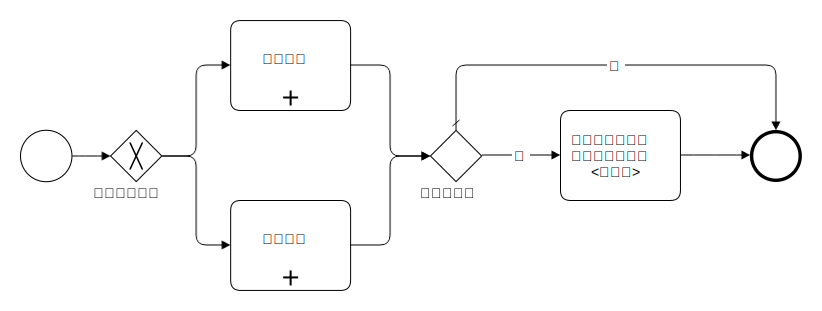
\includegraphics[width=\textwidth]{figures/bpm-cs.pdf}
    \caption{业务过程模型示意图(选课)\label{BPMCourseRegister}}
  \end{center}
\end{figure}

\begin{figure}[!hbp]
  \begin{center}
    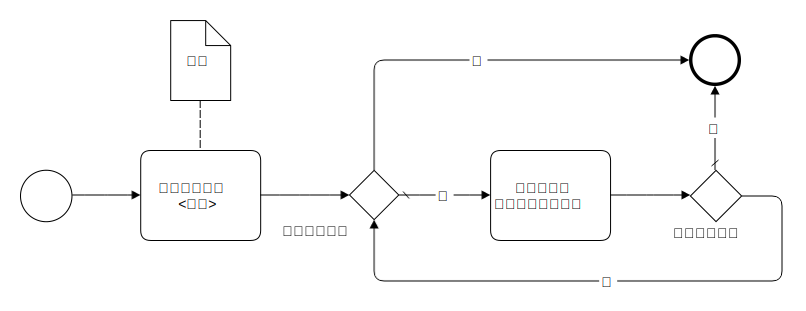
\includegraphics[width=\textwidth]{figures/bpm-cs-pref.pdf}
    \caption{业务过程模型示意图(选课-志愿)\label{BPMCourseRegisterP}}
  \end{center}
\end{figure}

\begin{figure}[!hbp]
  \begin{center}
    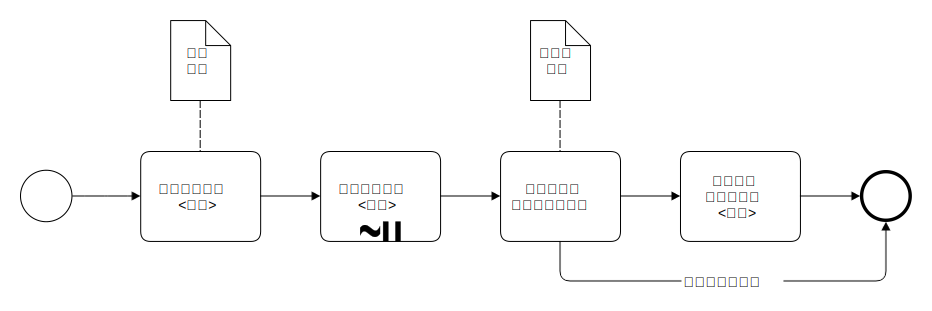
\includegraphics[width=\textwidth]{figures/bpm-cs-dual.pdf}
    \caption{业务过程模型示意图(选课-双选)\label{BPMCourseRegisterD}}
  \end{center}
\end{figure}

\begin{figure}[!hbp]
  \begin{center}
    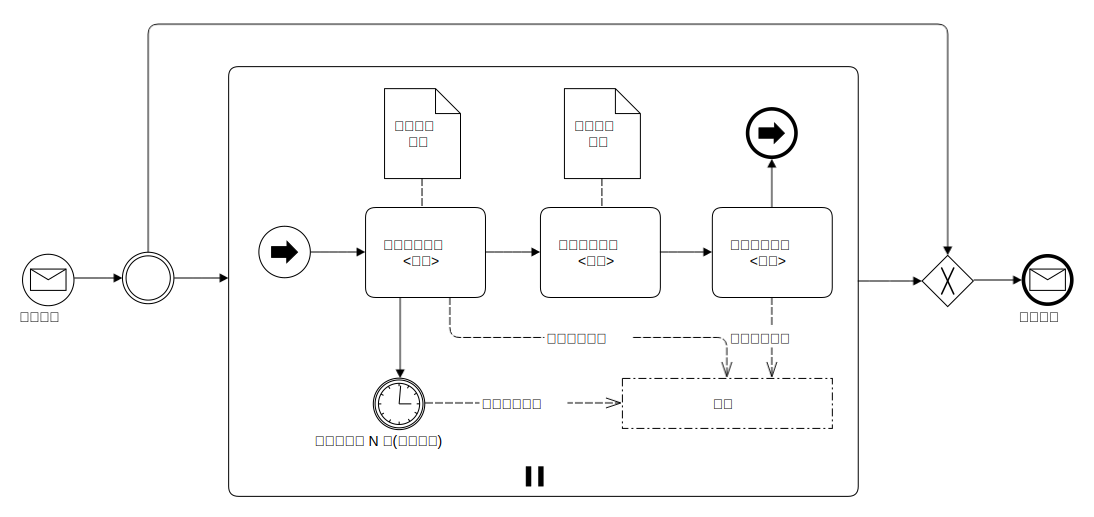
\includegraphics[width=\textwidth]{figures/bpm-task.pdf}
    \caption{业务过程模型示意图(课程任务)\label{BPMTask}}
  \end{center}
\end{figure}

\newpage

\section{课程管理系统产品需求表格}
\label{sec:appendix-requirement-table}

\LTXtable{\linewidth}{parts/table/requirement.tex}

\newpage

\section{数据库设计示意图}
\label{sec:appendix-database-diagram}

图~\ref{FullDatabaseDesign} 展示了完整的数据库设计视图:

\begin{figure}[!h]
  \begin{center}
    \includegraphics[angle=90, scale=0.5]{figures/eer-120dpi.png}
    \caption{数据库设计视图\label{FullDatabaseDesign}}
  \end{center}
\end{figure}

\newpage

\section{QueryBuilder 模块实现}

\verbatiminput{parts/code/querybuilder.js}

\newpage

\section{Entangle 核心实现}

\verbatiminput{parts/code/entangle.js}

% 恢复 TOC 设置 (本轮编译状态会被保存到下一轮)
\addtocontents{toc}{\protect\setcounter{tocdepth}{2}}

